\newcommand{\drive}
{
\begin{figure}[t]
\centering
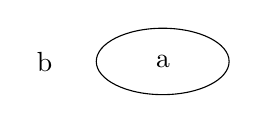
\begin{tikzpicture}[scale=1.5]
% \draw[draw=black, rounded corners=20pt] (0,0) rectangle (5,3);
\draw (0,0) ellipse (16pt and 8pt);
\draw (0,0) node {a};
\draw (-1, 0) node {b};
\end{tikzpicture}
\end{figure}
}

\newcommand{\organization}
{
\begin{figure}[t]
\centering
\begin{tikzpicture}[scale=1.5]
\draw (0,0) node {Задачи СХД};
\draw (-3,0) -- (-1,0);
\draw (3,0) -- (1,0);
\draw (-3,0) [-stealth]-- (-3, -0.85);
\draw (3,0) [-stealth]-- (3, -0.85)
\draw (-3,-1) node {Доступность};
\draw (3,-1) node {Надежность};
\draw (0, -1) node {Производительность};
\draw (0, -0.2) [-stealth]-- (0, -0.85);
\end{tikzpicture}
\end{figure}
}

\newcommand{\dma}
{
\begin{figure}[t]
\centering
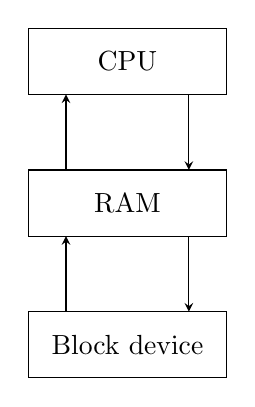
\begin{tikzpicture}[scale=.6]
\draw (0, 1) node {CPU};
\draw (0, -2) node {RAM};
\draw (0, -5) node {Block device};

\draw (-2.1, -4.3) rectangle (2.1, -5.7);
\draw (-2.1, -1.3) rectangle (2.1, -2.7);
\draw (-2.1, 1.7) rectangle (2.1, 0.3);


\draw (-1.3, -4.3) [-stealth]-- (-1.3,-2.7);
\draw (1.3, -4.3) [stealth-]-- (1.3,-2.7);

\draw (-1.3, -1.3) [-stealth]-- (-1.3, 0.3);
\draw (1.3, -1.3) [stealth-]-- (1.3, 0.3);
\end{tikzpicture}
\end{figure}
}

\newcommand{\nas}
{
\begin{figure}[t]
\centering
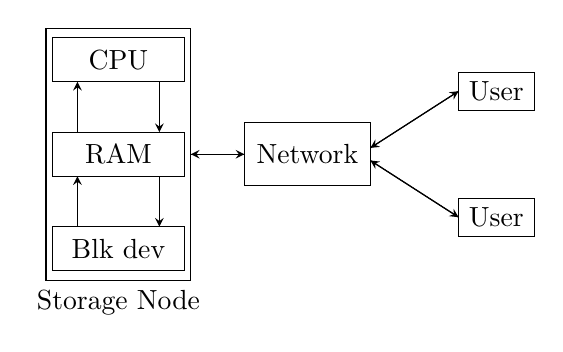
\begin{tikzpicture}[scale=.4]

\draw (-2.3, 2) rectangle (2.3, -6);
\draw (0, 1) node {CPU};
\draw (0, -2) node {RAM};
\draw (0, -5) node {Blk dev};
\draw (0, -6.7) node {Storage Node};

\draw (-2.1, -4.3) rectangle (2.1, -5.7);
\draw (-2.1, -1.3) rectangle (2.1, -2.7);
\draw (-2.1, 1.7) rectangle (2.1, 0.3);
\draw (-1.3, -4.3) [-stealth]-- (-1.3,-2.7);
\draw (1.3, -4.3) [stealth-]-- (1.3,-2.7);
\draw (-1.3, -1.3) [-stealth]-- (-1.3, 0.3);
\draw (1.3, -1.3) [stealth-]-- (1.3, 0.3);

\draw (2.3, -2) [stealth-]-- (4, -2);
\draw (2.3, -2) [-stealth]-- (4, -2);
\draw (6, -2) node {Network};
\draw (4, -1) rectangle (8 ,-3);

\draw (12, 0) node {User};
\draw (10.8, 0.6) rectangle (13.2, -0.6);
\draw (12, -4) node {User};
\draw (10.8, -3.4) rectangle (13.2, -4.6);

\draw (8, -1.8) [stealth-]-- (10.8, 0);
\draw (8, -1.8) [-stealth]-- (10.8, 0);

\draw (8, -2.2) [stealth-]-- (10.8, -4);
\draw (8, -2.2) [-stealth]-- (10.8, -4);

\end{tikzpicture}
\end{figure}
}

\newcommand{\bottleneck}
{
\begin{figure}[t]
\centering
\begin{tikzpicture}[scale=0.5]

\draw (0,0) [stealth-] -- (0, 13);

\draw (-0.5, 10) -- (0.5, 10);
\draw (-2.5, 10) node {\tiny 1999~г. SSE};

\node[align=left, anchor=west] at (1,11.5) 
    {CPU слабые и плохо справляются с логикой СХД\\ Логика СХД выносится в отдельный аппаратный контроллер \\(RAID-контроллер)};

\draw (-0.5, 5) -- (0.5, 5);
\draw (-2.5, 5) node {\tiny 2011~г. NVMe};

\node[align=left, anchor=west] at (1,7.5) 
    {На CPU появляются и развиваются векторные регистры \\ Бутылочным горлышком становится скорость операций с дисками \\ Логика на CPU позволяет внедрять дополнительную функциональность,\\ в том числе увеличивающую скорость операций};

\node[align=left, anchor=west] at (1,2.5) 
    {Появляются более быстрые диски и задачи в индустрии, для которых \\
    они необходимы (например запись видео высокого разрешения)\\
    Логика на CPU тормозит\\
    Ответ --- DPU (data processing unit)
    };



\end{tikzpicture}
\end{figure}
}

\newcommand{\stripe}
{
\begin{figure}[t]
\centering
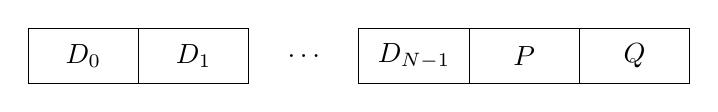
\begin{tikzpicture}[scale=0.7]

\draw (0,0) rectangle (2,1);
\draw (2,0) rectangle (4,1);
\draw (5,0.5) node {$\ldots$};
\draw (6,0) rectangle (8,1);
\draw (8,0) rectangle (10,1);
\draw (10,0) rectangle (12,1);

\draw (1,0.5) node {$D_0$};
\draw (3,0.5) node {$D_1$};
\draw (7,0.5) node {$D_{N-1}$};
\draw (9,0.5) node {$P$};
\draw (11,0.5) node {$Q$};

\end{tikzpicture}
\captionsetup{labelformat=empty}
\caption{Страйп RAID 6}
\end{figure}
}

\tikzset{radiation/.style={{decorate,decoration={expanding waves,angle=90,segment length=4pt}}},
         disk/.pic={
        code={\tikzset{scale=7/10}
            \draw (1,1) ellipse (1cm and 0.5cm);
            \draw (0,0) arc (180:360:1cm and 0.5cm);%
            \draw (0,-1) arc (180:360:1cm and 0.5cm);%
            \draw (0,-2) arc (180:360:1cm and 0.5cm);%
            \draw (0,-3) arc (180:360:1cm and 0.5cm);%
            
            \draw (0,1) -- (0,-3.05);
            \draw (2,1) -- (2,-3.05);
            \draw (1,1) -- (1,2);
  }}
}

\newcommand{\raid}
{
\begin{figure}[t]
\centering
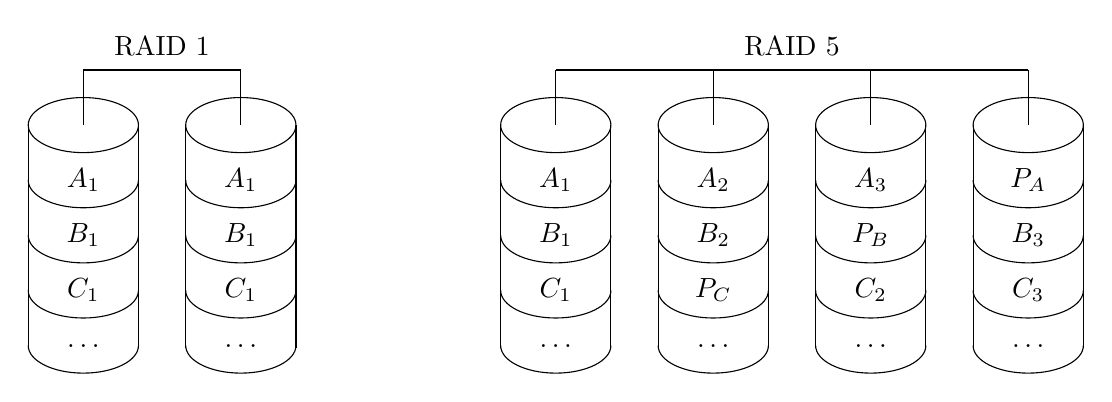
\begin{tikzpicture}

\path (0,0) pic {disk};
\path (2,0) pic {disk};
\draw (0.7,1.4) -- (2.7,1.4);
\draw (1.7 ,1.7) node {RAID 1};
\draw (0.7,0) node {$A_1$};
\draw (2.7,0) node {$A_1$};

\draw (0.7,-0.7) node {$B_1$};
\draw (2.7,-0.7) node {$B_1$};

\draw (0.7,-1.4) node {$C_1$};
\draw (2.7,-1.4) node {$C_1$};

\draw (0.7,-2.1) node {$\ldots$};
\draw (2.7,-2.1) node {$\ldots$};


\path (6,0) pic {disk};
\path (8,0) pic {disk};
\path (10,0) pic {disk};
\path (12,0) pic {disk};
\draw (6.7,1.4) -- (12.7,1.4);
\draw (9.7 ,1.7) node {RAID 5};


\draw (6.7,0) node {$A_1$};
\draw (8.7,0) node {$A_2$};
\draw (10.7,0) node {$A_3$};
\draw (12.7,0) node {$P_A$};

\draw (6.7,-0.7) node {$B_1$};
\draw (8.7,-0.7) node {$B_2$};
\draw (10.7,-0.7) node {$P_B$};
\draw (12.7,-0.7) node {$B_3$};

\draw (6.7,-1.4) node {$C_1$};
\draw (8.7,-1.4) node {$P_C$};
\draw (10.7,-1.4) node {$C_2$};
\draw (12.7,-1.4) node {$C_3$};

\draw (6.7,-2.1) node {$\ldots$};
\draw (8.7,-2.1) node {$\ldots$};
\draw (10.7,-2.1) node {$\ldots$};
\draw (12.7,-2.1) node {$\ldots$};

\end{tikzpicture}

\end{figure}
}


\newcommand{\raidPerf}
{
\begin{figure}[t]
\centering
\begin{tikzpicture}

\path (0,0) pic {disk};
\path (2,0) pic {disk};
\draw (0.7,1.4) -- (2.7,1.4);
\draw (1.7 ,1.7) node {RAID 1};
\draw (1.7 ,-3) node {Зеркалирование, может ускорять чтение};
\draw (0.7,0) node {$A_1$};
\draw (2.7,0) node {$A_1$};

\draw (0.7,-0.7) node {$B_1$};
\draw (2.7,-0.7) node {$B_1$};

\draw (0.7,-1.4) node {$C_1$};
\draw (2.7,-1.4) node {$C_1$};

\draw (0.7,-2.1) node {$\ldots$};
\draw (2.7,-2.1) node {$\ldots$};


\path (6,0) pic {disk};
\path (8,0) pic {disk};
\path (10,0) pic {disk};
\path (12,0) pic {disk};
\draw (6.7,1.4) -- (12.7,1.4);
\draw (9.7 ,1.7) node {RAID 0};
\draw (9.7 ,-3) node {Страйпинг, ускоряет чтение и запись};


\draw (6.7,0) node {$A_1$};
\draw (8.7,0) node {$A_2$};
\draw (10.7,0) node {$A_3$};
\draw (12.7,0) node {$A_4$};

\draw (6.7,-0.7) node {$B_1$};
\draw (8.7,-0.7) node {$B_2$};
\draw (10.7,-0.7) node {$B_3$};
\draw (12.7,-0.7) node {$B_4$};

\draw (6.7,-1.4) node {$C_1$};
\draw (8.7,-1.4) node {$C_2$};
\draw (10.7,-1.4) node {$C_3$};
\draw (12.7,-1.4) node {$C_4$};

\draw (6.7,-2.1) node {$\ldots$};
\draw (8.7,-2.1) node {$\ldots$};
\draw (10.7,-2.1) node {$\ldots$};
\draw (12.7,-2.1) node {$\ldots$};

\end{tikzpicture}

\end{figure}
}

\newcommand{\writehole}
{
\begin{figure}[t]
\centering
\begin{tikzpicture}[scale=0.5]

% \draw (0,0) rectangle (20,1);

\draw (0,0) rectangle (3.1,1);
\draw (1.55, -0.85) node {$D_1$};
\draw (1.55,1.2) [stealth-]-- (1.55, 2.5);
\draw[align=left, anchor=west] (1.6,2) node {Запись};

\draw[fill=green] (0.1,0.1) rectangle (0.3,0.9);
\draw[fill=green] (0.4,0.1) rectangle (0.6,0.9);
\draw[fill=green] (0.7,0.1) rectangle (0.9,0.9);
\draw[fill=green] (1,0.1) rectangle (1.2,0.9);
\draw(1.3,0.1) rectangle (1.5,0.9);
\draw (1.6,0.1) rectangle (1.8,0.9);
\draw (1.9,0.1) rectangle (2.1,0.9);
\draw (2.2,0.1) rectangle (2.4,0.9);
\draw (2.5,0.1) rectangle (2.7,0.9);
\draw (2.8,0.1) rectangle (3,0.9);

\draw (3.4, 0) rectangle (6.5,1);
\draw (4.95, -0.85) node {$D_2$};
\draw (4.95,1.2) [stealth-]-- (4.95, 2.5);
\draw[align=left, anchor=west] (5,2) node {Запись};


\draw[fill=green] (3.5,0.1) rectangle (3.7,0.9);
\draw[fill=green] (3.8,0.1) rectangle (4,0.9);
\draw[fill=green] (4.1,0.1) rectangle (4.3,0.9);
\draw[fill=green](4.4,0.1) rectangle (4.6,0.9);
\draw[fill=green] (4.7,0.1) rectangle (4.9,0.9);
\draw[fill=green] (5,0.1) rectangle (5.2,0.9);
\draw[fill=green] (5.3,0.1) rectangle (5.5,0.9);
\draw[fill=green] (5.6,0.1) rectangle (5.8,0.9);
\draw[fill=green] (5.9,0.1) rectangle (6.1,0.9);
\draw[fill=green] (6.2,0.1) rectangle (6.4,0.9);

% \draw (3.4, 0) rectangle (6.5,1);
\draw (6.8, 0) rectangle (9.9,1);
\draw (8.35, -0.85) node {$D_3$};


\draw (10.3,0) rectangle (13.4, 1);
\draw (11.85,1.2) [stealth-]-- (11.85, 2.5);
\draw[align=left, anchor=west] (11.9,2) node {Запись};
\draw (11.85,-0.85) node {$P$};
\draw[fill=green] (10.4,0.1) rectangle (10.6, 0.9);
\draw (10.7,0.1) rectangle (10.9, 0.9);
\draw (11,0.1) rectangle (11.2, 0.9);
\draw (11.3,0.1) rectangle (11.5, 0.9);
\draw (11.6,0.1) rectangle (11.8, 0.9);
\draw (11.9,0.1) rectangle (12.1, 0.9);
\draw (12.2,0.1) rectangle (12.4, 0.9);
\draw (12.5,0.1) rectangle (12.7, 0.9);
\draw (12.8,0.1) rectangle (13, 0.9);
\draw (13.1,0.1) rectangle (13.3, 0.9);


\end{tikzpicture}

\end{figure}
}

\newcommand{\san}
{
\begin{figure}[t]
\centering
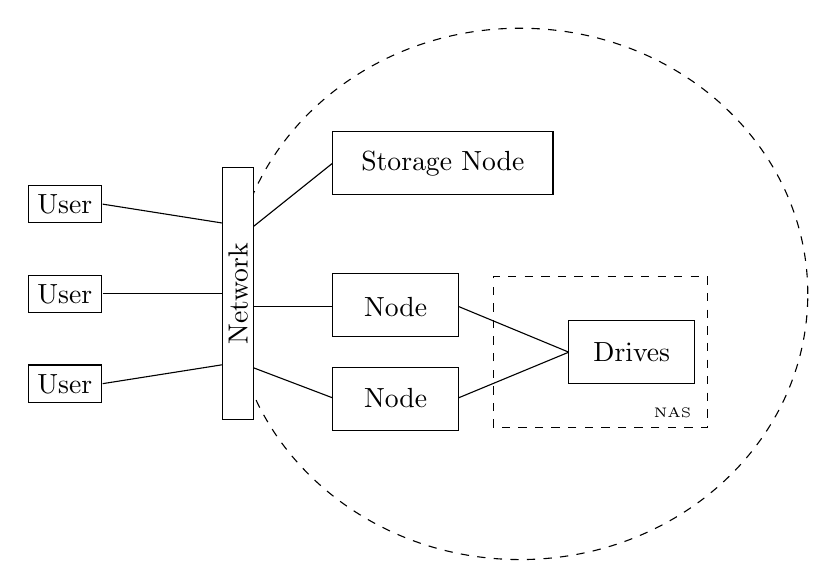
\begin{tikzpicture}[scale=0.8]


% \draw (1, 0.5) node {Network}; 



\draw (3.25, 1.75) rectangle (5.25, 0.75);
\draw (4.25, 1.225) node {Node};

\draw (3.25, -0.75) rectangle (5.25, 0.25);
\draw (4.25, -0.225) node {Node};

% NAS
\draw (7, 0) rectangle (9, 1);
\draw (8, 0.5) node {Drives}; 
\draw[dashed] (5.8, -0.7) rectangle (9.2, 1.7);
\draw[anchor=south east] (9.1,-0.7) node {\tiny NAS};

% \draw (3,-5) rectangle (8,-2);



% \draw (3,-1) rectangle (8,2);

\draw (3.25, 3) rectangle (6.75, 4);
\draw (5, 3.5) node {Storage Node};

% \draw () elipse
\draw[dashed] (6.225,1.425) ellipse (130pt and 120pt);
\draw[fill=white] (1.5, -0.575) rectangle (2,3.425);
\node[rotate=90] (Nw) at (1.75, 1.425) {Network};

\node[draw] (u1) at (-1,0) {User};
\node[draw] at (-1,1.425) {User};
\node[draw] at (-1,2.85) {User};

%user- - nw
\draw (-0.4, 2.85) -- (1.5, 2.55);
\draw (-0.4, 1.425) -- (1.5, 1.425);
\draw (-0.4, 0) -- (1.5, 0.3);


\draw (5.25, -0.225) -- (7, 0.5);
\draw (5.25, 1.225) -- (7, 0.5);

\draw (3.25, -0.225) -- (2, 0.25);
\draw (3.25, 1.225) -- (2, 1.225);

\draw (3.25, 3.5) -- (2, 2.5);

\end{tikzpicture}

\end{figure}
}
